\chapter {Diseño}

\section{Arquitectura objetivo}
\subsection{Servidores Físicos}
\begin{text}
	Al trabajar en una empresa de hosting, he tenido la suerte de contar con 3 servidores bare metal para el desarrollo de este proyecto. Las características técnicas de los servidores se pueden consultar en \nameref{servidores_bare_metal}.
\end{text}
\subsection{Infraestructura objetivo}
\begin{text}
	Este proyecto pretende crear una infraestructura para una pequeña empresa que se dedique al desarrollo del software. Esta infraestructura debe ser segura, con lo que ha de proporcionar firewalls redundantes y algún mecanismo para proporcional alta disponibilidad en las aplicaciones web.  A continuación se muestra la infraestructura objetivo. Cabe destacar que las Ips y la información que se muestra en la figura es únicamente de este proyecto con los dominios e IPs contratadas. Sin embargo, la red LAN dentro del cluster sí que se mantendría en otros despliegues del cluster, ya que está no depende de servicios externos. La siguiente figura muestra la estructura general de la infraestructura. Sin embargo, es necesario un nivel de abstracción más bajo para conocer los distintos servicios desplegados en el cluster bajo la red \textbf{10.6.0.0/16}.
	
	\clearpage
	
	\begin{figure}[!hbt]
		\label{InfraestructuraObjetivo}
		\centering
		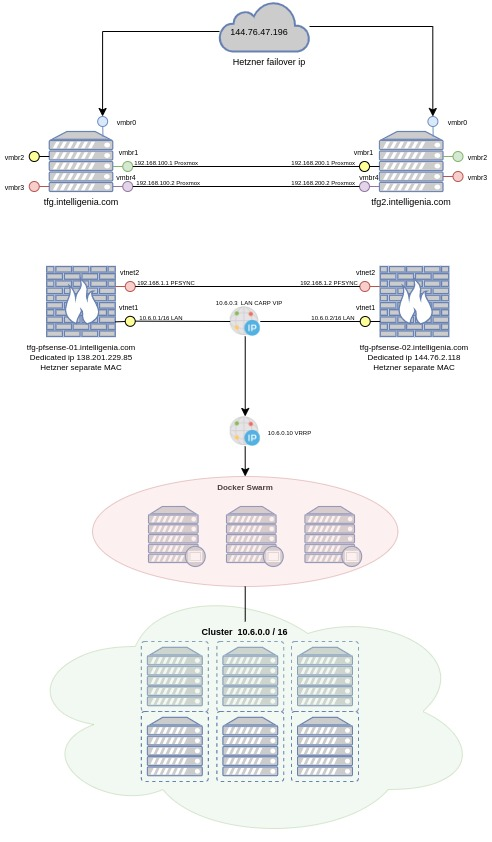
\includegraphics[scale=0.75]{imagenes/Analisis/diagrama.jpg}
		\caption[Infraestructura Objetivo]{Infraestructura Objetivo}
	\end{figure}
\end{text}

\clearpage

\subsection{VSwitch}
\begin{text}
	El cluster está bajo la red LAN 10.6.0.0/16, de forma que todas las máquinas virtuales están comunicadas. Sin embargo los nodos principales (tfg.intelligenia.com, tfg2.intelligenia.com y tfg3.intelligenia.com) tienen que estar comunicados a través de una red interna para el correcto funcionamiento de Proxmox y los pfSense.
	Es aquí donde entran en juego los switches virtuales de Hetzner. Un VSwitch simula el funcionamiento de un switch convencional, conectando los servidores que se conecten al switch entre sí. De este modo, conseguimos crear una red de conexión entre los nodos principales.
	
	\begin{figure}[!hbt]
		\centering
		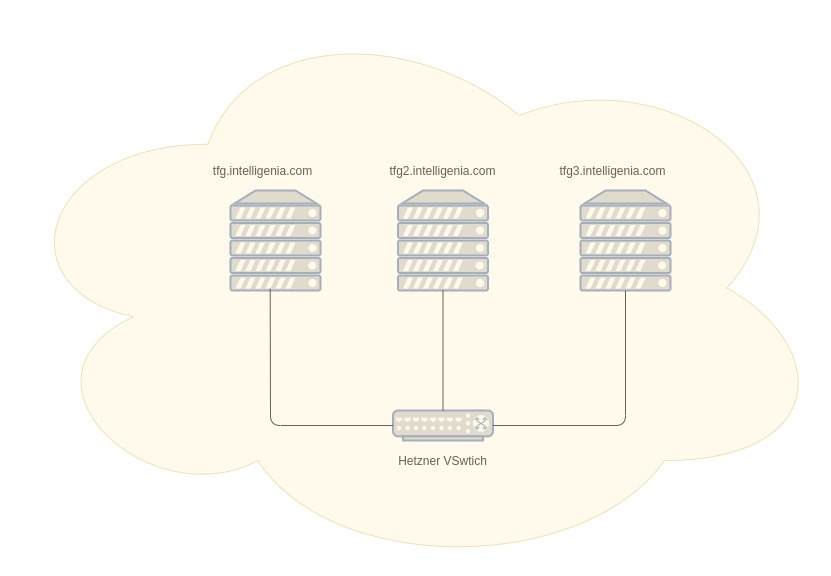
\includegraphics[scale=0.4]{imagenes/Analisis/vswitch.jpg}
		\caption[VSwitch]{VSwitch}
		\label{VSwitch}
	\end{figure}
\end{text}

\begin{text}
	La infraestructura anterior junto con los cauces pertinentes para la integración y despliegues continuos, es lo que pretende este proyecto. A continuación se explica como se ha diseñado la solución que satisface los requisitos funcionales relacionados con lac reación y despliegue de infraestructura con la herramienta de automatización Ansible.
\end{text}
\clearpage

\subsection{Diagrama Cluster}

\begin{text}
	La siguiente figura muestra el cluster con un nivel de abstracción más bajo. Se muestran los distintos servicios que ofrece el cluster y la relación entre ellos. Cada servicio desplegado contribuye a la realización de uno o más requisitos funcionales descritos en la sección \nameref{requisitosfuncionales} cucho propósito es lograr los objetivos definidos en \nameref{subobjetivos}. \\
	El cluster de servicios está interconectado entre sí en la red \textbf{10.6.100.0/24}.
\end{text}
\begin{figure}[!hbt]
	\centering
	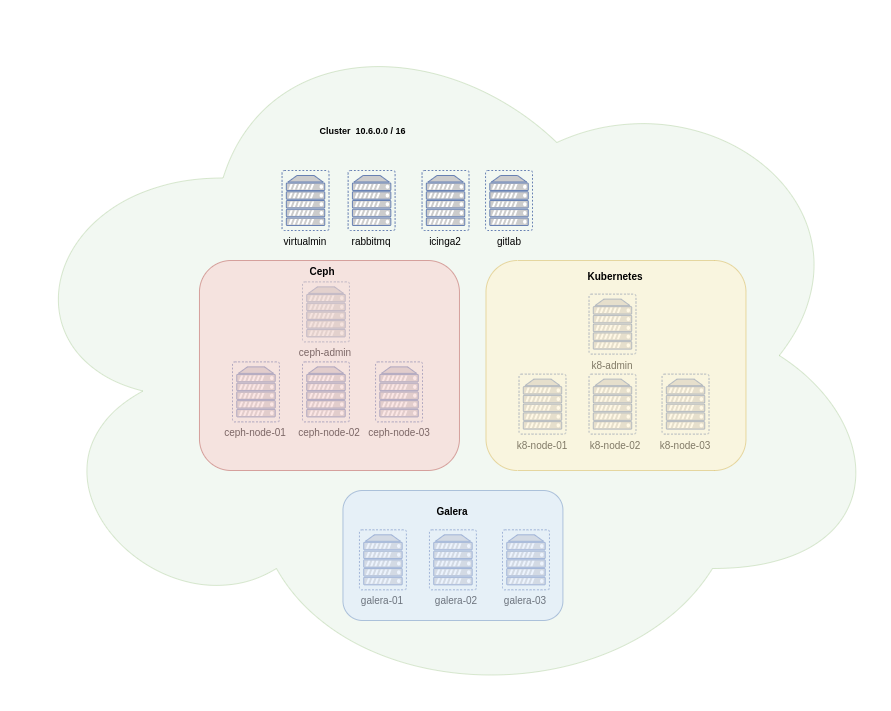
\includegraphics[scale=0.40]{imagenes/Diseno/diagrama_cluster_2.png}
	\caption[Diseño Cluster]{Diseño Cluster} 
	\label{cluster_design}
\end{figure}

\subsection{Servicios en cluster}

\subsubsection{Proveedor Infraestructura}
\begin{text}
	La infraestructura necesaria para formar el ecosistema que cumpla con los objetivos de este proyecto, se ha de alojar en servidores físicos. Para cumplir esta necesidad se ha elegido el proveedor Hetzner \cite{hetzner:online}, uno de los proveedores de servidores bare metal más conocidos en Europa. \\
\end{text}

\subsubsection{Servicio Virtualización}
\begin{text}
	Para poder ofrecer todos los servicios descritos en \nameref{objetivos_primarios} y cumplir con la arquitectura objetivo \nameref{Infraestructura_objetivo}, se hace necesario añadir una capa de virtualización a los servidores contratados. Estos 3 servidores físicos, servirán para desplegar los servicios descritos, sin embargo es necesario separar estos servicios en distintas máquinas. El servicio de virtualización nos permitirá crear tantas máquinas virtuales como servicios, virtualizando el hardware del servidor físico y aportando entornos cerrados, virtualizados y fácilmente recreables. \\
	El servicio de virtualización elegido ha sido Proxmox VE \cite{proxmox:online}, basado en KVM (Kernel-based Virtual Machine) y de código abierto. Se ha elegido este servicio de virtualización ya que es un requisito impuesto por la empresa.
\end{text}

\subsubsection{Firewall}
\begin{text}
	Hoy en día, con el auge de la informática y de las nuevas tecnologías, cada vez se están dando más y más ciberataques. Los denominados 'hackers' o delincuentes, aprovechan brechas de seguridad en los sistemas para poder hacerse con información sensible y después poder pedir rescate por dicha información. Estos ataques suelen aprovechar puertos abiertos, servicios obsoletos y vulnerabilidades conocidas para perpetrar sus ataques. Por ejemplo, esta web nos muestra en tiempo real la cantidad de ataques que sufre un país determinado \cite{ciberataques:online}.
	\begin{figure}[!hbt]
		\centering
		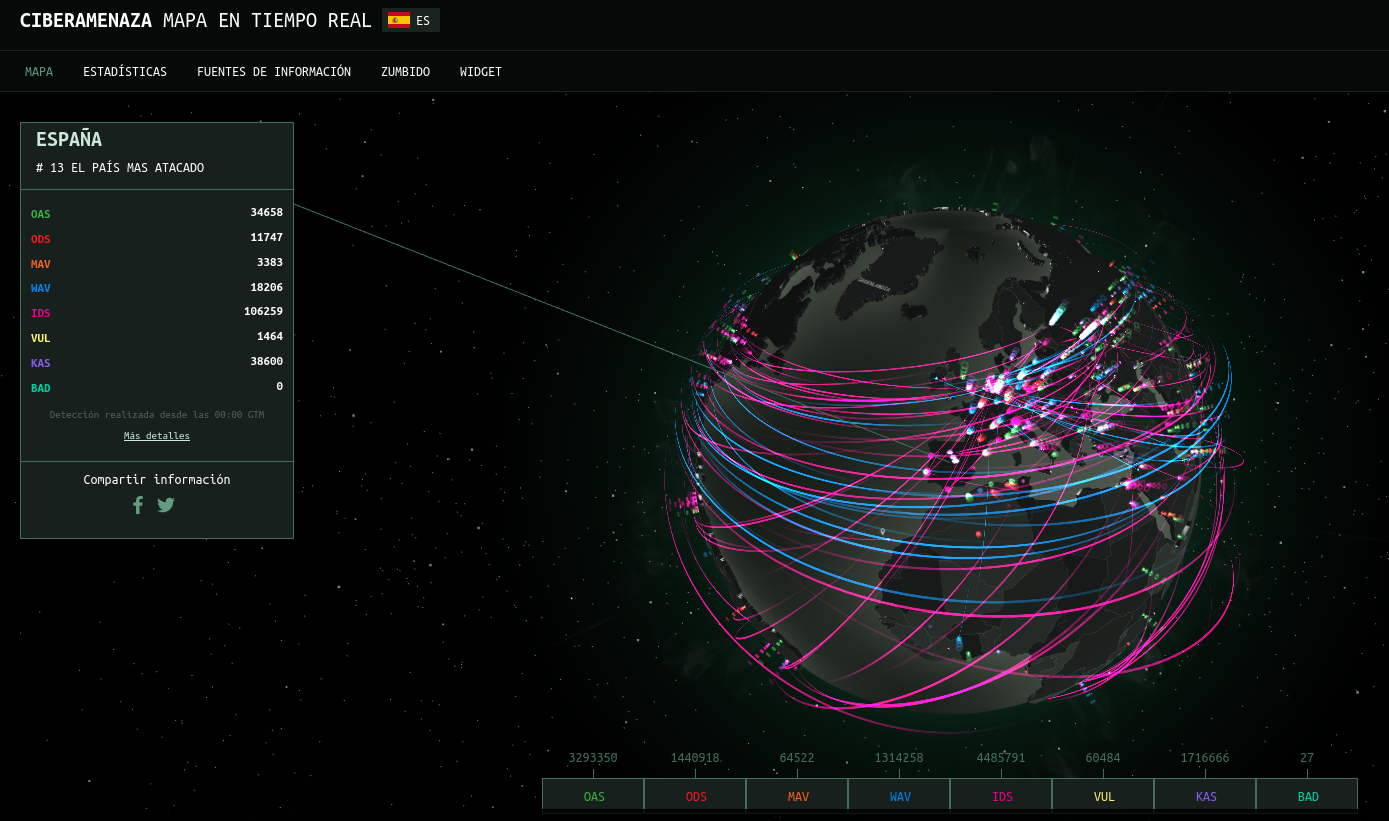
\includegraphics[scale=0.3]{imagenes/Diseno/ciberataques.png}
		\caption[Ciberataques]{Ciberataques \cite{ciberataques:online}} 
		\label{Ciberataques}
	\end{figure}
	Es por esto que se hace necesaria la protección de la infraestructura final, exponiendo únicamente los puertos necesarios para desviar el tráfico y trabajar con los servicios únicamente dentro de la red LAN segura. \\
	Para este fin se ha elegido la tecnología pfSense \cite{pfsense:online}. PfSense dispone de su versión community gratuita y de código abierto. Esta tecnología se ha elegido ya que es la tecnología utilizada en el cluster de producción de la empresa y es un requisito.
\end{text}

\subsubsection{Contenedores}
\begin{text}
	Como ya hemos visto, Proxmox nos proporciona una capa de virtualización del hardware de los servidores para poder crear máquinas virtuales donde alojar los distintos servicios. \\
	Sin embargo, a la hora del desarrollo y despliegue de aplicaciones web en el cluster, se hace inviable crear una máquina virtual por cada una de las aplicaciones web creadas. Esto sería insostenible ya que las máquinas virtuales demandan recursos. \\
	
	Para solventar este problema se van a crear aplicaciones en contenedores. Cada aplicación tendrá uno o varios contenedores dependiendo de los servicios, normalmente 1 servicio 1 contenedor. Para realizar este proceso se ha elegido la tecnología Docker. \cite{docker:online}.
\end{text}

\begin{text}
	Docker es la tecnología más famosa para crear contenedores. Gracias a Docker podemos aislar las aplicaciones en contenedores seguros y fácilmente replicables. Se ha elegido Docker por su extensa comunidad y porque es la tecnología más utilizada para este fin. Sin embargo, con esto no es suficiente ya que, una vez tengamos la aplicación separada en contenedores, necesitamos un entorno donde lanzar estos contenedores y poder gestionarlos. Es aquí donde surgen los orquestadores de contenedores. A continuación se hace una pequeña a dos orquestadores: Docker Swarm \cite{swarm:online} y Kubernetes \cite{k8:online}.
\end{text}

\subsubsection{Orquestación contenedores}
\begin{itemize}
	\item \textbf{Docker Swarm}. Docker Swarm es un software de orquestación de contenedores. Es la solución nativa de Docker para la gestión de los contenedores. Docker Swarm nos permite automatizar los procesos de despliegue escalado y gestión de contenedores. Sin embargo, cuando hablamos de escalado vertical o horizontal, Docker Swarm, al contrario que Kubernetes, no permite este escalado asegurando la disponibilidad. Debemos relanzar los contenedores con los nuevos parámetros para el escalado. \\
	Se ha elegido esta tecnología por ser la usada en un principio en la empresa para la gestión de contenedores. Cabe destacar que, aunque no ofrece los mismos servicios que Kubernetes, Docker Swarm es una solución muy buena para la orquestación de contenedores y su principal ventaja frente a Kubernetes es la facilidad para desplegar y gestionar los contenedores.
	\item \textbf{Kubernetes}. Kubernetes es un software de orquestación de contenedores que nos permite automatizar el proceso de despliegue, escalado y gestión de las aplicaciones en contenedores. Kubernetes se ha convertido en la solución principal para grandes empresas por su robustez. La principal ventaja de Kubernetes frente a sus competidores es la posibilidad de modificar las condiciones de escalado vertical o horizontal de los contenedores sin afectar a la disponibilidad de la aplicación. Su gran desventaja es la complejidad, ya que para poder manejar de forma eficiente un cluster de Kubernetes debemos pasar por un largo camino de aprendizaje. \\
	Se ha elegido esta tecnología por su gran demanda en el sector y como proceso de aprendizaje. Esta tecnología no estaba implementada en la empresa, sin embargo, se va a introducir como orquestador adicional.
\end{itemize}

\subsubsection{Almacenamiento estático}
\label{ceph}
\begin{text}
	Si bien tanto Docker Swarm como Kubernetes nos permiten gestionar los contenedores, estas tecnologías están pensadas para aplicaciones stateless o sin estado \cite{stateless:online}. A grandes rasgos, esto quiere decir que tanto Kubernetes como Docker Swarm, funcionan bien con aplicaciones que no necesitan almacenar información para su correcto funcionamiento. \\
	Para esto, Docker ofrece una solución en forma de volúmenes. Sin embargo, esta solución no se adecua a las necesidades de un entorno de alta disponibilidad  y alta fiabilidad. Es por esto que surge la necesidad de crear alguna solución de almacenamiento distribuido que nos proporcione dichas características. La solución elegida ha sido Ceph \cite{ceph:online}. Una vez más el uso de Ceph es un requisito impuesto por la empresa.
\end{text}
	
\subsubsection{Servidor Web / Proxy}
\begin{text}
	Para el correcto acceso de los clientes y desarrolladores a las aplicaciones, se hace necesario un proxy que desvíe las peticiones a la aplicación correcta. Para este fin se ha elegido la tecnología Nginx \cite{nginx:online}, que sirve a la vez de servidor web y de proxy. Un proxy es esencial para asegurar la seguridad del cluster, ya que únicamente hay un punto de entrada protegido por un proxy que a su vez está protegido por el firewall. De esta forma se aumenta la seguridad y se dificultan los intentos de ataque masivos. Se ha elegido Nginx por ser el usado en la empresa. Forma parte de los requisitos del proyecto impuestos por la empresa.
\end{text}

\subsubsection{Control de versiones}
\label{gitlab}
\begin{text}
	Para el correcto desarrollo del software y en este caso de la infraestructura, es necesario disponer de un servicio de control de versiones donde subir el código y llevar un seguimiento del mismo. Esto es muy importante, ya que cualquier cambio en el código queda reflejado y hacer rollbacks a versiones anteriores es posible. Para este fin se ha elegido la herramienta basada en git GitLab \cite{gitlab:online}. La elección de esta herramienta satisface los requisitos impuestos por la empresa.
\end{text}


\subsubsection{Base de datos}
\begin{text}
	Las aplicaciones lanzadas tanto en Docker Swarm como en Kubernetes, necesitarán almacenar el estado de la aplicación así como datos necesarios para el correcto funcionamiento de esta. Estos datos deben ser persistentes y no borrarse ante el reinicio de los contenedores o re-despliegue. Para esto, es necesario tener una base de datos que nos proporcione almacenamiento para las aplicaciones. La tecnología elegida para esta causa ha sido MariaDB, ya que las aplicaciones necesitan bases de datos relacionales y MariaDB está licenciado por GNU General Public License, así que lo podemos usar sin problemas. También se ha elegido esta tecnología porque es con la que más familiarizados estamos todos en la empresa. \\
	Para garantizar la alta disponibilidad y alto rendimiento a la hora de recuperar datos, se ha optado por la creación de un cluster de Galera \cite{galeracluster:online} con 3 nodos, uno en cada nodo principal de Proxmox. El uso de Galera forma parte de los requisitos impuestos por la empresa.
\end{text}

\section{Diseño de la solución basado en Ansible}
\begin{text}
	Como se ha discutido en la sección \nameref{tecnologias_elegidas} hemos elegido Ansible para cumplir los objetivos de este proyecto. Ansible nos permite automatizar el proceso de creación y configuración de la infraestructura. En la siguiente sección se hace un análisis de como se ha ido construyendo la solución utilizando Ansible en términos de metodología y forma de estructura el proyecto.
\end{text}

\subsection{Estructura, modularización y metodología}
\begin{text}
	Para diseñar la estructura y la metodología a seguir en el desarrollo se ha partido de los \nameref{requisitosfuncionales}. Para entender la metodología utilizada hay que conocer como funciona Ansible.
	
	\subsubsection{Ansible}
	\label{ansible_}
	\begin{text}
		Ansible es una herramienta de automatización que nos permite lanzar playbooks contra servidores remotos o locales.
		\begin{itemize}
			\item \textbf{Playbooks}: un playbook consiste en un conjunto de tareas que se ejecutan de forma secuencial en los hosts definidos. Sin embargo, los playbooks por si solos aportan poca flexibilidad a la hora de estructurar los proyectos y dificulta la comprensión de estos ya que se pueden convertir en ficheros muy largos difíciles de seguir. Es por esto que surge la necesidad de organizar de algún modo las tareas por funcionalidad. Es aquí donde surgen los roles.
			
			\item \textbf{Roles:}: un role nos permite agrupar múltiples tareas bajo un mismo nombre. Por ejemplo, podríamos crear un role llamado firewall en el cual definiríamos todas las tareas que involucren al firewall. Ésto hace que el proyecto sea más legible y ayuda al futuro desarrollo.
		\end{itemize}
	
	Para cada caso de uso definido en \nameref{casosdeuso} se ha creado un playbook. En nuestro caso, hemos creado un role para cada servicio desplegado en el cluster. Estos roles harán los playbooks más legibles. \\
	En cada role se definen una serie de variables para decidir qué tareas se van a lanzar. Para explicar esto pongamos el ejemplo del role \textbf{webproxy}. Este role tiene varias tareas:
	\begin{itemize}
		\item \textbf{apply\_config.yml}
		\item \textbf{create\_site.yml}
		\item \textbf{create\_ssl\_cert.yml}
		\item \textbf{install\_certbot.yml}
		\item \textbf{install\_nginx.yml}
	\end{itemize}

	Podría darse el caso que quisieramos crear un sitio en nginx sin certificado SSL. Para esto se han definido unas variables que se han de definir en cada playbook para elegir qué tareas lanzar de cada role. \\
	Cada tarea definida en los role, corresponde con un issue definido en \nameref{issues}.
	
	\clearpage
	
	A continuación se listan los distintos playbooks definidos y se relacionan con sus correspondientes \nameref{requisitosfuncionales} e \nameref{issues}.
	
	\begin{itemize}
		\item \textbf{configure\_local\_environment.yml}. \hyperref[RF0]{RF0}.
		\begin{itemize}
			\item Issue 0.1 - 0.2.
		\end{itemize}
	
		\item \textbf{configure\_proxmox\_node.yml}. \hyperref[RF1]{RF1}, \hyperref[RF4]{RF4}.
		\begin{itemize}
			\item Issue 1 - 1.10.
		\end{itemize}
	
		\item \textbf{apply\_config\_pfsense.yml}. \hyperref[RF3]{RF3}, \hyperref[RF4]{RF4}.
		\begin{itemize}
			\item Issue 2.3.
		\end{itemize}
	
		\item \textbf{deploy\_pfsense\_firewall.yml}. \hyperref[RF3]{RF3}, \hyperref[RF4]{RF4}.
		\begin{itemize}
			\item Issue 2.1,2.2,2.4.
		\end{itemize}
		
		\item \textbf{create\_gitlab.yml}. \hyperref[RF3]{RF3}, \hyperref[RF4]{RF4}.
		\begin{itemize}
			\item Issue 3.1 - 3.4.
		\end{itemize}
	
		\item \textbf{create\_ceph\_cluster.yml}. \hyperref[RF3]{RF3}, \hyperref[RF4]{RF4}.
		\begin{itemize}
			\item Issue 5.1.
		\end{itemize}
	
		\item \textbf{create\_virtualmin.yml}. \hyperref[RF3]{RF3}, \hyperref[RF4]{RF4}.
		\begin{itemize}
			\item Issue 5.3.
		\end{itemize}
	
		\item \textbf{create\_webproxy.yml}. \hyperref[RF3]{RF3}, \hyperref[RF4]{RF4}.
		\begin{itemize}
			\item Issue 5.6.
		\end{itemize}
	
		\item \textbf{create\_icinga2.yml}. \hyperref[RF3]{RF3}, \hyperref[RF4]{RF4}.
		\begin{itemize}
			\item Issue 4.1 - 4.4.
		\end{itemize}
	
		\item \textbf{create\_galera\_cluster.yml}. \hyperref[RF3]{RF3}, \hyperref[RF4]{RF4}.
		\begin{itemize}
			\item Issue 5.2.
		\end{itemize}
	
		\item \textbf{create\_rabbitmq.yml}. \hyperref[RF3]{RF3}, \hyperref[RF4]{RF4}.
		\begin{itemize}
			\item Issue 5.5.
		\end{itemize}
	
		\item \textbf{create\_docker\_swarm\_cluster.yml}. \hyperref[RF3]{RF3}, \hyperref[RF4]{RF4}.
		\begin{itemize}
			\item Issue 5.7.
		\end{itemize}
		\item \textbf{create\_kubernetes\_cluster.yml}. \hyperref[RF3]{RF3}, \hyperref[RF4]{RF4}.
		\begin{itemize}
			\item Issue 5.7.
		\end{itemize}
		
	\end{itemize}

	\end{text}
\end{text}

\subsection{Despliegue solución}
\begin{text}
	Una vez diseñada e implementada la solución su despliegue consiste en ejecutar los distintos playbooks en la infraestructura objetivo. Sin embargo, antes de poder lanzar estos playbooks, hay que configurar un fichero \textbf{hosts.yml} donde definimos los hosts donde desplegar el proyecto así como la distribución de servicios en los nodos y otra información como la IP de cada servicio. \\
	Una vez realizada la configuración pertinente, el único requisito por parte de la empresa es el alquiler de 2 o más servidores (bare metal) en Hetzner \cite{hetzner:online}.
\end{text}

\subsection{Cumplimiento requisitos funcionales}
\begin{text}
	Al haber estructurado el proyecto creando un playbook o más por cada requisito funcional, y al tener cada role definidos una serie de test, si se cumple el objetivo de cada playbook, se cumplirán los requisitos funcionales. \\
	Como hemos comentado en la sección \nameref{ansible_}, Ansible se encarga de ejecutar las tareas definidas en los roles y en los playbooks de forma secuencial. Cada tarea de Ansible tiene un objetivo el cual si no se cumple, se lanza una excepción en forma de error abortando la ejecución del playbook. Esta forma de funcionar nos asegura que, si un playbook de los definidos en este proyecto termina su ejecución con éxito, los issues a los que está asociado dicho playbook van a quedar resueltos.
\end{text}

\section{Posibles mejoras}
        \begin{text}
                El proyecto que describe este documento, es una solución integral para resolver el problema de infraestructura en una pequeña empresa. Si hablamos de posibles mejoras, ya que siempre se puede mejorar, hablaríamos de hacer más eficientes los playbooks de Ansible o estructurarlos de forma que sean más comprensibles si cabe. Cabe destacar que en el diseño del cluster se incluye un cluster de Kubernetes, el cual está justamente para mejorar el cluster de docker-swarm. \\
                Un punto importante de mejora sería implementar las técnicas de integración continua y entrega continua a las aplicaciones Wordpress de Virtualmin, ya que en este proyecto únicamente se abordan los proyectos Django + Angular de la empresa. \\
                A grandes rasgos y exceptuando pequeñas mejoras en la calidad del código o la documentación, pienso que el proyecto es muy ambicioso y está bien diseñado a nivel de infraestructura, no necesitando grandes cambios en un futuro próximo.
        \end{text}